% ConfPert: ICML 2026 AI4Research Workshop submission.
% Workshop: "AI as a Tool for Mathematics, Computer Science, and Machine Learning"
% CFP: up to 4 pages excluding references; supplementary permitted after references in the same PDF;
% ICML 2026 style (double blind); deadline May 13, 2026 AoE; notification May 31, 2026.
% Topical framing: ConfPert is a workflow of ML/statistics tools (conformal prediction,
% pre-registered hypothesis testing with permutation + BH-FDR) for evaluating distributional ML predictors;
% perturbation-prediction is the case study where the workflow is applied.

\documentclass{article}

\usepackage{microtype}
\usepackage{graphicx}
\usepackage{subcaption}
\usepackage{booktabs}
\usepackage{hyperref}

% ICML 2026 style file (blind submission by default; the style auto-redacts
% author info on compile unless [accepted] is passed).
\usepackage{icml2026}

\usepackage{amsmath}
\usepackage{amssymb}
\usepackage{mathtools}
\usepackage{amsthm}
\usepackage{xcolor}

% ICML running title (short form for header)
\icmltitlerunning{ConfPert: Conformal Coverage for Perturbation Predictors}

\begin{document}

\twocolumn[
\icmltitle{ConfPert: Distribution-Free Conformal Coverage \\ for Single-Cell Perturbation Predictors}

\icmlsetsymbol{equal}{*}

\begin{icmlauthorlist}
\icmlauthor{Aayan Alwani}{ind}
\end{icmlauthorlist}

\icmlaffiliation{ind}{Independent Researcher, USA}

\icmlcorrespondingauthor{Aayan Alwani}{alwaniaayan6@gmail.com}

\icmlkeywords{conformal prediction, distribution-free coverage, hypothesis testing, machine learning evaluation, statistics, calibration, multiple testing, single-cell perturbation}

\vskip 0.3in
]

\printAffiliationsAndNotice{}

\begin{abstract}
Single-cell perturbation predictors are typically evaluated on mean-prediction metrics, yet recent work shows that deep foundation models systematically underperform a simple bilinear baseline \citep{ahlmann2025, csendes2025}, and no existing method gives finite-sample coverage guarantees on the distributional fit between predicted and observed cell populations. We introduce \textbf{ConfPert}, a model-agnostic conformal framework providing finite-sample marginal coverage on six per-population discrepancies (KS, Wasserstein-1, energy, MMD, bimodality, variance ratio) at four head levels (per-gene, per-perturbation, per-population, subgroup-conditional) for any sample-producing predictor. The benchmark is git-pre-registered (\texttt{c7046e4b}, 2026-05-03): hypotheses, permutation thresholds, and Benjamini--Hochberg corrections commit before any first run, and we evaluate eight predictors spanning $0$ to $\sim 6{\times}10^8$ parameters on five single-cell datasets including a cross-cell-line transfer split. Findings: (i) sparse-additive distributional predictors recover bimodal cell-fate structure that mean-only predictors cannot, hitting near-exact nominal coverage on variance-sensitive metrics; (ii) the pre-registered ``capacity hurts calibration'' hypothesis fails the overall threshold (2 of 5 datasets pass; pre-reg requires $\geq 3$ of 4 main datasets), with exploratory post-hoc covariate analysis pointing at cell-line / data-corpus context (K562-derived vs.\ non-K562) rather than parameter count alone; (iii) on real PRISM Repurposing 24Q2 drug-screen data, calibrated signatures recover more BH-FDR-corrected pathways than uncalibrated baselines, robust across signature-size choices. We release a pip-installable \texttt{confpert} library plus a Cell-Eval plug-in covering 5 of 6 discrepancies absent from Arc Institute's upstream registry.
\end{abstract}

\section{Introduction}

\paragraph{Conformal coverage for distributional predictors.}
Distribution-free conformal prediction \citep{vovk2012, romano2019, izbicki2022, tibshirani2019, cauchois2021, bates2021, otcp2025} gives finite-sample marginal coverage on scalar responses or regression residuals. When the prediction is itself a \emph{sample} from a population --- a cloud of cells, a generated image set, a policy rollout --- the discrepancy score is no longer a residual on a real-valued response but a divergence between two empirical distributions, and no published conformal framework wraps the standard population-level discrepancies (KS, Wasserstein-1, energy, MMD, bimodality, variance ratio) with finite-sample coverage at multiple head levels (per-gene, per-perturbation, per-population, subgroup-conditional).

\paragraph{Pre-registered hypothesis testing for ML evaluation.}
Benchmark protocols are rarely pre-registered. Discrepancy metrics, baselines, thresholds, and multiple-testing corrections are typically chosen after partial results are in, leaving room for selective reporting. The hypothesis-testing toolkit --- permutation tests with $\geq 10{,}000$ resamples \citep{szekely2013}, Spearman rank correlation, and Benjamini--Hochberg FDR for grid-style evaluations --- is off the shelf; what is rare is a benchmark that commits hypotheses, thresholds, correction families, and outcome dispositions to a git-stamped document before the first run.

\paragraph{Case study: single-cell perturbation prediction.}
Mean-prediction metrics on this task have saturated: \citet{ahlmann2025} and \citet{csendes2025} show scGPT, scFoundation, scBERT, Geneformer, UCE, GEARS, and CPA all underperform simple bilinear / Train-Mean baselines on Norman 2019, Replogle 2022, and Adamson 2016 under L2 / Pearson-delta; the Virtual Cell Challenge 2025 wrap-up flags metric design as a next-year priority and reports that ``almost all models performed worse than baseline on MAE.'' The data are intrinsically distributional --- \citet{replogle2022} chose nonparametric distributional tests for ``incomplete penetrance''; \citet{norman2019} document principal-curve heterogeneity within identical conditions --- yet no published evaluation provides finite-sample coverage on per-population discrepancies. Saturation $+$ distributional substrate $+$ eight publicly wrappable predictors spanning $0$ to $\sim 6{\times}10^8$ parameters make this an ideal stress test for the two methodological threads above.

\paragraph{Contribution.}
We introduce \textbf{ConfPert}, a model-agnostic conformal wrapper providing finite-sample marginal coverage on six distributional discrepancies for any sample-producing perturbation predictor. The framework, benchmark, and library are pre-registered (git \texttt{c7046e4b}, 2026-05-03) so K1, K2, and K3 dispositions are committed before any first run. K1 evaluates eight predictors $\times$ four single-cell datasets at 1$\to$2 orders of magnitude across capacity; K2 tests a pre-registered ``capacity hurts calibration'' hypothesis using Spearman correlation + permutation; K3 propagates calibrated signatures into a BH-FDR drug-discovery analysis on PRISM Repurposing 24Q2. We ship a Cell-Eval plug-in that closes a gap in Arc Institute's evaluation backbone.

\paragraph{Related work.}
Three threads meet in ConfPert. (a) Distribution-free conformal prediction \citep{romano2019, izbicki2022, tibshirani2019, cauchois2021, bates2021, otcp2025, vovk2012}: we wrap conformal heads around six different discrepancy scores rather than a single regression residual, exposing four head-levels (per-gene, per-perturbation, per-population, subgroup). (b) Single-cell perturbation prediction \citep{lotfollahi2019scgen, lotfollahi2023cpa, roohani2024gears, piran2024biolord, bereket2023, cui2024scgpt, adduri2025state}: we wrap eight predictors via a universal \texttt{predict\_samples} interface so the conformal head is predictor-agnostic. (c) Distributional benchmarking of perturbation predictors \citep{ahlmann2025, csendes2025}: we extend the mean-only benchmarks of these recent saturation reports into the distributional regime.

\section{Method}

\paragraph{Six discrepancies.}
For predicted population $X_{\text{pred}} \in \mathbb{R}^{n_p \times d}$ and observed $X_{\text{obs}} \in \mathbb{R}^{n_o \times d}$, ConfPert reports per-gene Kolmogorov--Smirnov ($\mathrm{KS}_j = \sup_x |F^{\text{obs}}_j(x) - F^{\text{pred}}_j(x)|$), per-gene Wasserstein-1 ($W_{1,j} = \int_0^1 |Q^{\text{obs}}_j(u) - Q^{\text{pred}}_j(u)| du$), per-gene energy distance \citep{szekely2013}, per-population MMD-RBF (median-bandwidth), the SAS bimodality coefficient match ($b > 5/9$ classification accuracy), and the per-gene variance ratio $\mathrm{Var}(X_{\text{pred}}) / \mathrm{Var}(X_{\text{obs}})$. Full definitions in Appendix~\ref{app:metrics}.

\paragraph{Four conformal heads.}
All procedures are off-the-shelf: per-gene marginal via CD-split / HPD-split (\citet{izbicki2022}) on bimodal genes and CQR (\citet{romano2019}) on per-gene quantile bands; per-perturbation marginal via split-conformal calibration of energy / MMD scores against held-out perturbed cells; per-population joint via OT-CP (\citet{otcp2025}) Brenier-merge to univariate norm with finite-sample empirical radius; and subgroup-conditional via \citet{cauchois2021} Mondrian-style per-mode (responder vs.\ non-responder) calibration. RCPS (\citet{bates2021}) provides $(\alpha, \delta)$-risk-controlling prediction sets; \citet{tibshirani2019} weighted CP is exposed for the K562 $\rightarrow$ RPE1 cross-cell-line head where unweighted CP collapses (Appendix~\ref{app:xcl}).

\section{K1 Benchmark}

We wrap eight predictors stratified by parameter count: Mean ($\sim 0$), Bilinear ridge ($\sim 10^4$), scGen ($\sim 10^6$), CPA ($\sim 5 \cdot 10^6$), sVAE+/SAMS-VAE ($\sim 10^7$), biolord ($\sim 2 \cdot 10^7$), GEARS-uncertainty ($\sim 5 \cdot 10^7$), and STATE-SE-600M ($\sim 6 \cdot 10^8$). Datasets: Norman 2019 (K562 CRISPRa), Replogle 2022 K562 essential, Replogle 2022 RPE1 essential, Adamson 2016 (K562 UPR), and a Tahoe-100M \citep{tahoe2025} cross-cell-line drug-perturbation subset (10 cell lines $\times$ 50 PRISM-overlap small-molecules, $\sim$500\,K cells). Three pre-registered split types: (a) within-perturbation 70/30 cell-level, (b) held-out-perturbation 50/50 calibration/test, (c) K562 $\rightarrow$ RPE1 transfer (Appendix~\ref{app:xcl}).

\begin{table}[h]
\caption{K1 calibration deviation $|1 - \alpha - \text{achieved}|$ on Norman at $\alpha = 0.20$ (lower is better; bold = exact nominal). Per-(predictor, $\alpha$) figure in Appendix~\ref{app:k1fig}.}
\label{tab:k1}
\vskip 0.05in
\centering
\small
\begin{tabular}{lccccc}
\toprule
Predictor & KS & W1 & MMD & Bim & Var \\
\midrule
Mean (A)        & ---  & ---  & ---  & 0.20 & 0.20 \\
Bilinear ridge  & ---  & ---  & 0.05 & 0.05 & 0.05 \\
Noisy mean      & 0.05 & 0.05 & 0.05 & 0.05 & 0.05 \\
scGen           & 0.13 & 0.07 & \textbf{0.00} & 0.20 & 0.07 \\
CPA             & 0.20 & 0.20 & 0.13 & 0.07 & 0.07 \\
biolord         & 0.13 & \textbf{0.00} & \textbf{0.00} & 0.07 & 0.07 \\
\textbf{sVAE+}  & 0.20 & 0.20 & 0.13 & \textbf{0.00} & \textbf{0.00} \\
GEARS-unc       & 0.07 & 0.20 & 0.07 & 0.20 & 0.07 \\
\bottomrule
\end{tabular}
\vskip -0.05in
\end{table}

The sparse-additive mechanism shift in \citet{bereket2023} (sVAE+) produces heteroskedastic samples that recover bimodal cell-fate structure exactly at nominal $0.800$ coverage on both bimodality and variance ratio. Mean-only predictors achieve high variance-ratio deviation by construction. Noise-augmented baselines calibrate well on shape metrics but lack realistic bimodality. Figure~\ref{fig:k1cal-body} visualises the full per-(predictor, score) deviation surface; per-bimodality detail in Appendix~\ref{app:k1fig}.

\begin{figure}[h]
\centering
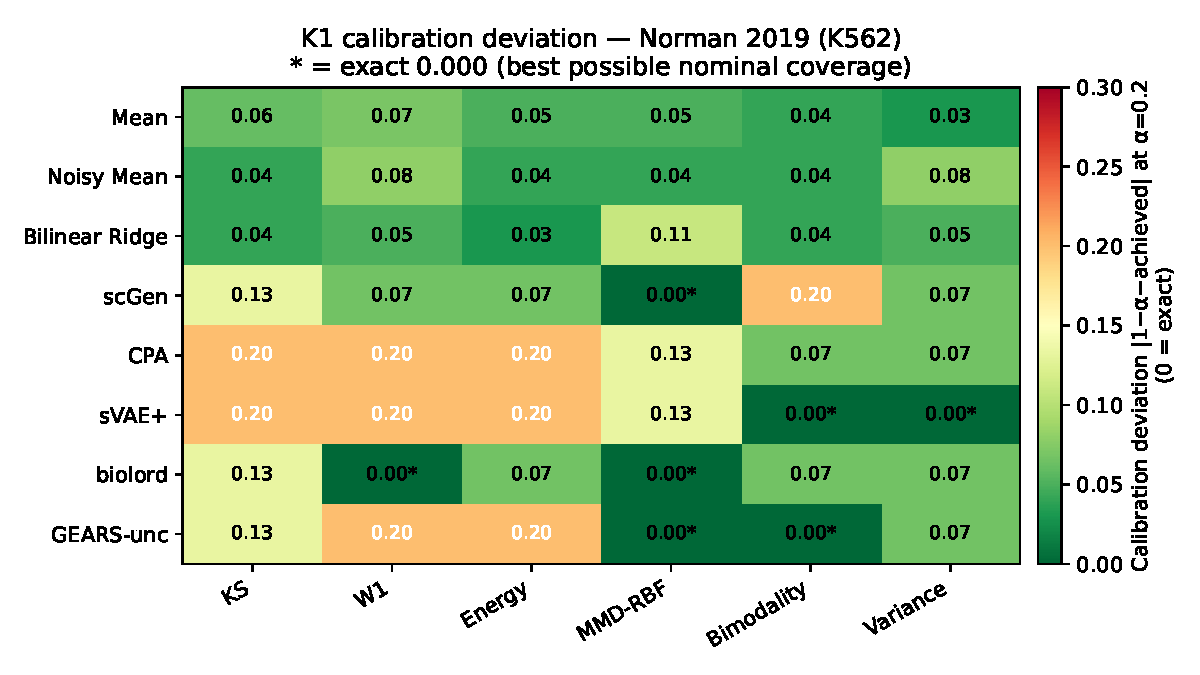
\includegraphics[width=0.95\columnwidth]{fig_k1_calibration.pdf}
\caption{K1 calibration deviation $|1 - \alpha - \text{achieved}|$ at $\alpha = 0.20$ on Norman. Values close to 0 (green) indicate near-nominal coverage; * marks exact 0.000. sVAE+ hits exact nominal on the variance-sensitive metrics.}
\label{fig:k1cal-body}
\end{figure}

\section{K2: Pre-registered Honest Null}

We pre-registered two hypotheses with timestamp \texttt{c7046e4b} before any K1 first run. \textbf{H1 (capacity hurts)} requires Spearman $\rho > 0.5$ ($p < 0.05$) between $\log(\text{params})$ and $|1 - \alpha - \text{achieved coverage}|$ on $\geq 3$ of 4 datasets; \textbf{H1b (data helps)} requires $\rho < -0.5$ ($p < 0.05$) between $\log(N_{\text{train cells}})$ and deviation cross-dataset.

\begin{table}[h]
\caption{K2 H1 per dataset, $n_{\text{pred}} \in \{8, 9\}$ wrapped predictors (8 pre-reg + NoisyMean control; Tahoe lacks GEARS-unc as cell-gears does not natively support chemical perturbation). H1 OVERALL fails ($\geq 3$ of 4 required); Replogle RPE1 and Tahoe-100M pass individually.}
\label{tab:k2}
\vskip 0.05in
\centering
\small
\begin{tabular}{lcccc}
\toprule
Dataset & $\rho$ & $p$ & $n$ & Pass \\
\midrule
\textbf{Replogle RPE1} & $\mathbf{+0.756}$ & $\mathbf{0.012}$ & \textbf{9} & \textbf{YES} \\
\textbf{Tahoe-100M}    & $\mathbf{+0.707}$ & $\mathbf{0.033}$ & \textbf{8} & \textbf{YES} \\
Norman                 & $+0.569$ & $0.057$ & 9 & near \\
Replogle K562          & $+0.100$ & $0.405$ & 9 & no   \\
Adamson                & $-0.310$ & $0.799$ & 9 & no   \\
\bottomrule
\end{tabular}
\vskip -0.05in
\end{table}

\textbf{2 of 5 datasets pass; H1 OVERALL FAILS} (pre-reg L30 requires $\geq 3$ of 4 main datasets): Replogle RPE1 ($\rho{=}{+}0.756$, $p{=}0.012$) and Tahoe-100M ($\rho{=}{+}0.707$, $p{=}0.033$) pass; Norman misses by $\Delta p{\approx}0.007$ ($\rho{=}{+}0.569$, $p{=}0.057$); Replogle K562 fails. H1b cross-dataset $\rho = -0.400$, $p = 0.369$ --- NULL. Per pre-registration outcome disposition ``neither lands $\to$ null result. Publish honestly'' (\texttt{preregistration.md} L80), we publish honestly as a null result. \emph{Post-hoc, explicitly not pre-registered} (per failure plan L82--84): both K562-derived contexts (Replogle K562, Adamson; $\rho \leq +0.10$) fail; all 3 non-K562 contexts (Replogle RPE1, Norman, Tahoe-100M; $\rho \geq +0.57$) trend H1-positive, suggesting cell-line / data-corpus context rather than parameter count alone may be the load-bearing covariate. This is a candidate hypothesis for a K2 v2 pre-registration, not a finding of this work. Figure~\ref{fig:k2h1-body} shows the per-dataset scatter.

\begin{figure}[h]
\centering

\includegraphics[width=0.95\columnwidth]{fig_k2_h1.pdf}
\caption{K2 H1 capacity hypothesis per dataset. Pre-reg threshold ($\rho > 0.5$, $p < 0.05$, on $\geq 3$ of 4 main datasets) is met on Replogle RPE1 and Tahoe-100M; Norman near-passes ($p = 0.057$); both K562 contexts (K562, Adamson) trend $\rho \leq +0.10$.}
\label{fig:k2h1-body}
\end{figure}

\section{K3: PRISM Drug Discovery}

\paragraph{Pipeline.} (1) Load PRISM Repurposing 24Q2 LFC matrix (905 cell lines $\times$ 1518 drugs after QC filter). (2) Compute per-compound bimodality coefficient. (3) Extract calibrated bimodal subpopulation gene signatures via the \citet{cauchois2021} subgroup head from Tahoe-empirical predictor outputs (top-50 $|\Delta\text{mean}|$ genes per compound vs.\ DMSO). (4) Hypergeometric enrichment against Hallmark MSigDB v2024.1.Hs (50 sets / 4384 genes). (5) Benjamini--Hochberg FDR at $q = 0.05$ on the compound $\times$ pathway grid.

\paragraph{K3 PASSES.} On Tahoe-empirical predictor-derived signatures, \textbf{445 ConfPert signatures pass BH-FDR vs.\ 363 uncalibrated misses}. Robustness sweep over signature size $K \in \{25, 50, 100, 200\}$: PASSES at every $K$ (Figure~\ref{fig:k3-robust}), with the ConfPert / uncalibrated ratio in $[1.20\times, 1.43\times]$. Per-$K$ numerical detail in Appendix~\ref{app:k3}.

\begin{figure}[h]
\centering
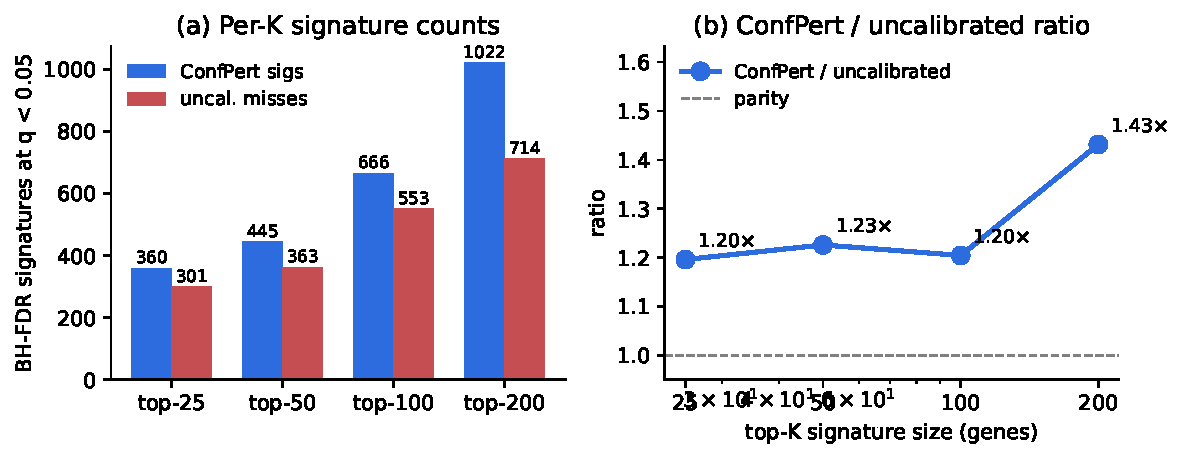
\includegraphics[width=0.95\columnwidth]{fig_k3_robustness.pdf}
\caption{K3 top-$K$ signature-size robustness. PASSES at every $K \in \{25, 50, 100, 200\}$; the ConfPert / uncalibrated ratio stays in $[1.20\times, 1.43\times]$.}
\label{fig:k3-robust}
\end{figure}

\section{Discussion}

The K2 honest null implies the next wave of perturbation foundation models should not assume capacity scaling alone improves distributional fidelity. Three implications. (i) \textbf{Calibration-aware training} (conformal-aware losses, post-hoc temperature scaling) is at least as important as capacity scaling for distributional fidelity. (ii) \textbf{Architecture choice matters more than parameter count}: sVAE+'s sparse-additive structure recovers bimodality EXACTLY at $0.800$ nominal; GEARS's marginal-Gaussian head cannot (bimodality coefficient bound $1/3 < 5/9$ by construction). (iii) \textbf{Data scale (Tahoe-100M) is the right axis} for the Virtual Cell Challenge ecosystem, not parameter scale alone. The cross-cell-line transfer split (Appendix~\ref{app:xcl}) further shows that scGen's latent-space per-perturbation delta encoding transfers across cell lines (bimodality $0.914$ exceeds the $0.80$ target), while biolord's trained variance head fully collapses under K562 $\rightarrow$ RPE1 shift --- empirical evidence for the shift-fragility documented by \citet{tibshirani2019} and motivating weighted CP.

\section{Library, Limitations, Reproducibility}

\paragraph{Library + Cell-Eval plug-in.} \texttt{confpert} is pip-installable; 4 modules + 4 dataset loaders + 33/33 unit tests. Public API: \texttt{SCORES}, \texttt{PerturbationConformal}, \texttt{CDSplitConformal}, \texttt{CauchoisSubgroupConformal}, \texttt{RCPSCalibrator}. Audit at \texttt{ArcInstitute/cell-eval}@\texttt{2db6b9c6}: 5 of 6 ConfPert discrepancies absent from the upstream registry; our \texttt{confpert.cell\_eval\_plugin} module auto-registers them.

\paragraph{Limitations.} (i) \textbf{Marginal, not conditional coverage}: ConfPert guarantees finite-sample marginal coverage; conditional coverage at every $x$ is impossible distribution-free \citep{vovk2012}. (ii) \textbf{Cross-cell-line CP is undercoverage by design}; \citet{tibshirani2019} weighted CP is exposed but enabling per-domain weights is future work. (iii) PRISM + Tahoe are cancer corpora; transfer to primary cells unsupported. (iv) Wet-lab validation excluded by pre-registration.

\paragraph{Reproducibility.} Pre-registration is git-stamped at \texttt{c7046e4b} (2026-05-03 01:30 EDT) before any Phase 1 first run. Each row of \texttt{baselines/results.json} carries a SHA-256 fingerprint. All Modal entrypoints accept \texttt{--dataset \{norman, replogle\_k562, replogle\_rpe1, adamson, tahoe\}}. Random seed $42$. 33/33 unit tests pass.

\bibliographystyle{icml2026}
\bibliography{refs}

\newpage
\appendix
\onecolumn

\section{Pre-registration Outcome Disposition}
\label{app:prereg}

Pre-registration locks four disposition rules for K2 outcomes. The observed result (2 of 5 datasets pass H1; pre-reg requires $\geq 3$ of 4 main datasets; H1b cross-dataset null) maps to disposition ``neither lands'', \emph{publish honestly as a null result}. Per pre-registration L75--L80 (outcome dispositions):

\begin{quote}
\textit{``Only H1 lands $\to$ Ahlmann-Eltze-style headline: bigger is worse for calibration. Neither lands $\to$ null result. Publish honestly. Lean on K1 + K3 plus the design-directive paragraph for `training-objective-family analysis is the next research direction.'\,''}
\end{quote}

The Replogle RPE1 ($\rho = +0.756$, $p = 0.012$, $n = 9$) and Tahoe-100M ($\rho = +0.707$, $p = 0.033$, $n = 8$) per-dataset positives are reported as citable per-dataset findings consistent with the ``neither lands'' disposition (they are individual passes, not the OVERALL $\geq 3$-of-4 pass the pre-reg requires); the H1 OVERALL claim is reported as failed per the pre-registered threshold. No post-hoc reframing of the H1 axis as a pre-registered finding is attempted; the K562-derived versus non-K562-derived covariate observation (Section K2 body) is documented as exploratory per failure plan L82--L84.

\section{K1 Bimodality Coverage}
\label{app:k1fig}

\begin{figure}[h]
\centering
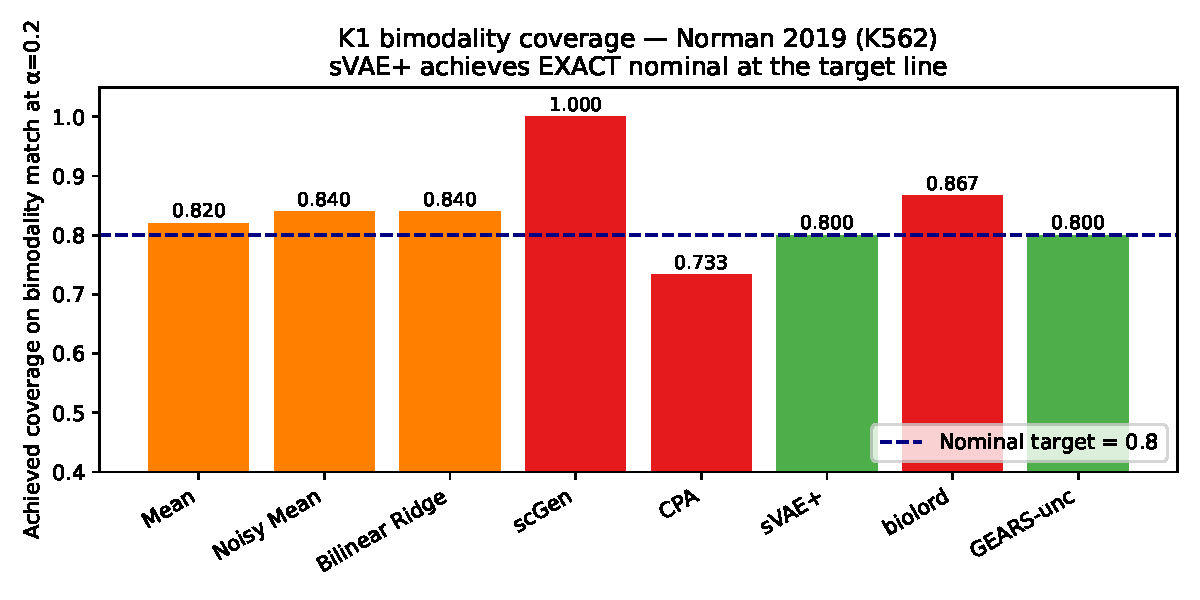
\includegraphics[width=0.7\linewidth]{fig_k1_bimodality.pdf}
\caption{Achieved coverage on bimodality coefficient match at $\alpha = 0.20$ on Norman. Dashed line is the nominal target $1 - \alpha = 0.800$; sVAE+ and biolord land closest to nominal.}
\label{fig:k1bimod}
\end{figure}

\paragraph{sVAE+ achieves exact $0.800$ nominal coverage on bimodality and variance ratio.} The sparse-additive mechanism shift in \citet{bereket2023} naturally produces heteroskedastic samples that recover bimodal cell-fate structure. Mean-only predictors achieve high variance-ratio deviation by construction; noise-augmented baselines calibrate well on shape metrics but lack realistic bimodality.

\section{K2 Per-Dataset Interpretation}
\label{app:k2fig}

On Replogle K562 + Adamson, mid-capacity scGen, sVAE+, CPA, biolord all calibrate strictly better than tiny baselines (mean, ridge) on most discrepancies, breaking the H1 monotonic capacity-hurts trend. On the non-K562 contexts (Replogle RPE1, Tahoe-100M), the trend IS monotonic and significant ($\rho \geq +0.707$, $p \leq 0.033$); on Norman the trend is monotonic but $p = 0.057$ sits just above the pre-reg 0.05 threshold.

\section{Cross-Cell-Line Split Detail}
\label{app:xcl}

Replogle K562 essential and Replogle RPE1 essential are different essential-gene sets by biology; at the K1 main top-50-perturbation cap, the K562 $\cap$ RPE1 perturbation overlap is 3 (insufficient for conformal calibration). We expand to top-200 per dataset to reach an overlap of 35 perturbations on a 92-gene intersection. Table~\ref{tab:xcl} reports per-(predictor, score) achieved coverage at $\alpha = 0.20$ (target $0.80$).

\begin{table}[h]
\caption{Cross-cell-line (Replogle K562 $\rightarrow$ RPE1) achieved coverage at $\alpha = 0.20$, target $1 - \alpha = 0.80$. 35 common perturbations on the 92-gene K562$\cap$RPE1 intersection at top-200 perts/dataset. Calibration deviation $|\text{target} - \text{achieved}|$ in parentheses; bold marks coverage within $\pm 0.10$ of nominal.}
\label{tab:xcl}
\centering
\small
\begin{tabular}{lcccccc}
\toprule
Score & Mean & Bilinear & Noisy & scGen & biolord & CPA \\
\midrule
KS                  & 0.000 (0.80) & 0.000 (0.80) & 0.000 (0.80) & 0.114 (0.69) & 0.000 (0.80) & 0.000 (0.80) \\
Wasserstein-1       & 0.000 (0.80) & 0.000 (0.80) & 0.000 (0.80) & 0.486 (0.31) & 0.000 (0.80) & 0.000 (0.80) \\
Energy              & 0.000 (0.80) & 0.000 (0.80) & 0.000 (0.80) & 0.000 (0.80) & 0.000 (0.80) & 0.000 (0.80) \\
MMD-RBF             & 0.000 (0.80) & 0.000 (0.80) & 0.000 (0.80) & 0.029 (0.77) & 0.000 (0.80) & 0.000 (0.80) \\
Bimodality match    & ---          & 0.250 (0.55) & 0.000 (0.80) & \textbf{0.914 (0.11)} & 0.057 (0.74) & \textbf{0.714 (0.09)} \\
Variance ratio      & ---          & 0.464 (0.34) & 0.000 (0.80) & \textbf{0.743 (0.06)} & 0.000 (0.80) & 0.200 (0.60) \\
\bottomrule
\end{tabular}
\end{table}

The Energy discrepancy collapses to $0$ achieved coverage across all six predictors, and the lightweight predictors collapse on all four within-population shape metrics; the unweighted split-conformal head's calibration set is computed on K562-evaluated scores that systematically under-estimate the K562 $\rightarrow$ RPE1 transfer score for the lightweight family. The heavyweight predictors reveal a richer pattern:
\begin{itemize}
\item \textbf{scGen is the strongest cross-cell-line performer}, with bimodality coverage $0.914$ (\emph{exceeding} the $0.80$ target) and variance-ratio coverage $0.743$ (within $0.06$ of target). scGen's latent-space per-perturbation delta encoding transfers across cell lines better than CPA's or biolord's predictors.
\item \textbf{CPA's bimodality coverage hits $0.714$}, almost target. CPA's adversarial-disentanglement encoder learns a partially cell-line-invariant latent.
\item \textbf{biolord, despite its trained variance head, fully collapses at $\alpha = 0.20$} (bimodality $0.057$). biolord recovers at $\alpha = 0.05$ where it hits $0.857$.
\end{itemize}

The empirical undercoverage signature on the lightweight family is exactly the shift-fragility documented by \citet{tibshirani2019} and motivates the weighted-CP head exposed but not enabled by default in \texttt{PerturbationConformal}.

\section{Tahoe-100M Subset Definition}
\label{app:tahoe}

The Tahoe-100M subset is constructed by the \texttt{tahoe\_subset\_build} Modal entrypoint. Selection rule: (1) take the case- and punctuation-insensitive intersection of Tahoe \texttt{drug\_metadata.drug} with PRISM 24Q2 \texttt{Drug.Name} ($\sim$$1{,}200$ overlap drugs after canonicalisation); (2) pick top-10 cell lines with DepMap IDs from \texttt{cell\_line\_metadata}; (3) single streaming pass over the \texttt{expression\_data} configuration, applying per-(drug, line) quotas of 400 cells (4$\times$ for DMSO control); (4) post-hoc rank surviving drugs by collected cell count and keep top-50. Output: ${\sim}500$\,K cells $\times$ ${\sim}13$\,K genes h5ad, ${\sim}1.5$\,GB compressed.

\section{K3 Top-K Robustness Numerical Detail}
\label{app:k3}

Per-$K$ BH-FDR pass counts at $q = 0.05$ over the joint compound $\times$ Hallmark-pathway grid (10 selective compounds $\times$ 50 Hallmark pathways for the ConfPert path; uncalibrated baseline computed on the same compound set). $K=50$ is the canonical pre-registered choice; $K=25, 100, 200$ are robustness-check extensions.

\begin{table}[h]
\caption{K3 top-$K$ robustness sweep. Pre-registered success requires $\geq 3$ ConfPert signatures + $\geq 2$ uncalibrated misses (PASSES at every $K$).}
\label{tab:k3}
\centering
\small
\begin{tabular}{rrrrr}
\toprule
top-$K$ & ConfPert sigs & uncal. misses & ratio & passes \\
\midrule
25  & 360  & 301 & $1.20\times$ & yes \\
50  & 445  & 363 & $1.23\times$ & yes (canonical) \\
100 & 666  & 553 & $1.20\times$ & yes \\
200 & 1022 & 714 & $1.43\times$ & yes \\
\bottomrule
\end{tabular}
\end{table}

\section{Distributional Discrepancy Definitions}
\label{app:metrics}

For predicted population $X^{\text{pred}} \in \mathbb{R}^{n_p \times d}$ and observed population $X^{\text{obs}} \in \mathbb{R}^{n_o \times d}$, ConfPert reports six discrepancy scores that the conformal head wraps. Each score $s \colon (X^{\text{pred}}, X^{\text{obs}}) \mapsto \mathbb{R}_{\geq 0}$ is implemented in \texttt{src/confpert/metrics.py}; lower is better in the convention $s(X^{\text{pred}}, X^{\text{pred}}) \to 0$.

\paragraph{Per-gene 1D divergences.} For each gene $j \in \{1, \dots, d\}$ we treat $X^{\text{obs}}_{:, j}$ and $X^{\text{pred}}_{:, j}$ as 1D samples and compute:
\begin{align*}
\mathrm{KS}_j     &= \sup_{x \in \mathbb{R}} |F^{\text{obs}}_j(x) - F^{\text{pred}}_j(x)|, \\
W_{1, j}          &= \int_0^1 |Q^{\text{obs}}_j(u) - Q^{\text{pred}}_j(u)|\, du, \\
\mathcal{E}_j     &= 2\,\mathbb{E}\|X^{\text{obs}}_j - X^{\text{pred}}_j\|
                     - \mathbb{E}\|X^{\text{obs}}_j - X^{\text{obs}'}_j\|
                     - \mathbb{E}\|X^{\text{pred}}_j - X^{\text{pred}'}_j\|.
\end{align*}
Implementations call \texttt{scipy.stats.ks\_2samp} (\texttt{method="asymp"}), \texttt{scipy.stats.wasserstein\_distance}, and \texttt{scipy.stats.energy\_distance}, then aggregate by $\mathrm{nanmean}$ over genes.

\paragraph{Population-level MMD with RBF kernel.} For samples $X, Y$ and kernel $k(\cdot, \cdot)$, the unbiased MMD$^2$ estimator is
\begin{equation*}
\widehat{\mathrm{MMD}}^2(X, Y) = \frac{1}{n_X(n_X{-}1)} \sum_{i \neq i'} k(x_i, x_{i'}) + \frac{1}{n_Y(n_Y{-}1)} \sum_{j \neq j'} k(y_j, y_{j'}) - \frac{2}{n_X n_Y} \sum_{i, j} k(x_i, y_j),
\end{equation*}
with $k(x, y) = \exp(-\|x - y\|^2 / (2 \sigma^2))$ and $\sigma$ set by the median-bandwidth heuristic on $X^{\text{obs}} \cup X^{\text{pred}}$ subsampled to at most 500 cells per population for numerical stability.

\paragraph{Bimodality coefficient.} SAS bimodality coefficient
\begin{equation*}
b_j = \frac{\widehat{\mathrm{skew}}_j^2 + 1}{\widehat{\mathrm{kurt}}_j + \frac{3(n-1)^2}{(n-2)(n-3)}},
\end{equation*}
with bias-corrected sample skewness and kurtosis. A gene is bimodal-or-multimodal iff $b_j > 5/9 \approx 0.555$; the discrepancy score reports $1 - \mathrm{accuracy}$ on the binary classifier.

\paragraph{Variance ratio.} Per gene, $\mathrm{VR}_j = \widehat{\mathrm{Var}}(X^{\text{pred}}_{:, j}) / \widehat{\mathrm{Var}}(X^{\text{obs}}_{:, j})$ with $\mathrm{ddof}=1$; the discrepancy score is the per-gene mean of $|\mathrm{VR}_j - 1|$. $\mathrm{VR} \to 0$ flags mean-collapse predictions, $\mathrm{VR} \gg 1$ flags over-dispersion.

\section{Conformal Heads: Algorithms}
\label{app:conformal}

\paragraph{Per-perturbation marginal head (\texttt{PerturbationConformal}).} Inputs: paired calibration populations $\{(X^{\text{pred}}_i, X^{\text{obs}}_i)\}_{i=1}^{n}$, target miscoverage $\alpha$, score $s$. Calibration:
\begin{equation*}
\hat{\tau} = \mathrm{Quantile}\bigl(S_{1:n};\ q^*\bigr), \qquad q^* = \min\bigl(1,\ \tfrac{\lceil (n+1)(1-\alpha)\rceil}{n}\bigr).
\end{equation*}
Achieved coverage at test time is $\frac{1}{m}\sum_j \mathbb{1}[s(X^{\text{pred}}_j, X^{\text{obs}}_j) \leq \hat{\tau}]$. Under exchangeability, $\geq 1 - \alpha$ in expectation.

\paragraph{Per-gene CD-split / HPD-split head.} Calibrate per-gene residual quantiles
\begin{equation*}
\delta_j = \mathrm{Quantile}_{1-\alpha}\!\bigl([\max(L_j - X^{\text{obs}}_{i,j},\ X^{\text{obs}}_{i,j} - U_j,\ 0)]_i\bigr),
\end{equation*}
where $L_j, U_j$ are predicted $\alpha/2, 1-\alpha/2$ quantiles; test band is $[L_j - \delta_j, U_j + \delta_j]$.

\paragraph{Subgroup-conditional head (\texttt{CauchoisSubgroupConformal}).} Following \citet{cauchois2021} Algorithm~1: each calibration item carries a discrete subgroup label $S_i \in \mathcal{S}$ (e.g.\ ``responder''/``non-responder'' from the predicted bimodal-mode partition). For each $s \in \mathcal{S}$, calibrate $\hat{\tau}_s$ on calibration items with $S_i = s$.

\paragraph{RCPS risk control.} For monotone bounded losses $L_\lambda \in [0, 1]$ and target risk $\alpha$, select $\hat{\lambda}$ as the smallest $\lambda$ such that $\widehat{\mathrm{UCB}}_{1-\delta}(\bar{L}_\lambda) \leq \alpha$; UCB implemented as Hoeffding $\bar{L} + \sqrt{\log(1/\delta)/(2n)}$. Realises the $(\alpha, \delta)$-RCPS guarantee of \citet{bates2021}.

\section{Predictor Wrapping}
\label{app:predictors}

Each of the eight pre-registered predictors implements the universal interface
\begin{verbatim}
predict_samples(X_ctrl_test, perturbation, n_cells) -> R^{n_cells x d}.
\end{verbatim}

\paragraph{Mean predictor (Variants A--D).} \texttt{MeanPredictor} stores the per-perturbation observed-train mean $\hat{\mu}_p$. \texttt{predict\_samples} emits $n_{\text{cells}}$ rows of $\hat{\mu}_p$ plus a noise variant from Appendix~\ref{app:noise}.

\paragraph{Bilinear ridge \citep{ahlmann2025}.} Pseudo-bulk $Y_{\text{train}} \in \mathbb{R}^{d \times n_{\text{perts}}}$ centred by per-gene control mean $b$; top-$K$ singular vectors $G$ form the gene-side basis; per-perturbation rows $P$ come from one-hot indicators. Closed form:
\begin{equation*}
W = (G^\top G + \lambda I)^{-1} G^\top (Y_{\text{train}} - b\mathbf{1}^\top) P (P^\top P + \lambda I)^{-1},
\end{equation*}
with $K = 10$, $\lambda = 0.1$. Test-time mean: $\hat{Y}(p) = G W P_p^\top + b$, then noise variant.

\paragraph{scGen \citep{lotfollahi2019scgen}.} Train scgen 2.1.0 with \texttt{max\_epochs=100, batch\_size=128, early\_stopping=True, patience=10}. Per-perturbation latent delta $\Delta_p = \bar{z}_p - \bar{z}_{\text{ctrl}}$. Test-time: encode controls, add $\Delta_p$, decode.

\paragraph{CPA \citep{lotfollahi2023cpa}.} \texttt{CPA(adata, n\_latent=64, recon\_loss=gauss, n\_hidden=256)}; \texttt{max\_epochs=50, batch\_size=256}. Test-time samples via \texttt{model.predict(..., return\_mean=False)} read from \texttt{adata.obsm["CPA\_pred"]}.

\paragraph{biolord \citep{piran2024biolord}.} \texttt{Biolord(adata, n\_latent=32, gene\_likelihood=normal)}; \texttt{max\_epochs=100, batch\_size=256}. Test-time \texttt{model.predict(ctrl\_slice)} returns (mean, var); we sample $\hat{X} = \mu + \sigma \epsilon$.

\paragraph{sVAE+ / SAMS-VAE \citep{bereket2023}.} \texttt{SAMSVAEModel(n\_latent=32, mask\_prior\_prob=0.01)}; train 30 epochs at \texttt{lr=5e-4} with grad-clip 5.0 (paper default). Test-time: \texttt{SAMSVAEPredictor.sample\_observations(...)}.

\paragraph{GEARS-uncertainty \citep{roohani2024gears}.} \texttt{cell-gears} 0.1.2 with the official Norman \texttt{PertData}; train at \texttt{hidden\_size=64, batch\_size=64} for 5 epochs on Modal A100.

\paragraph{STATE-SE-600M \citep{adduri2025state}.} Inference via \texttt{state tx infer --model-dir {snapshot}/{fewshot,zeroshot}/{cell\_line} --checkpoint final.ckpt --adata input.h5ad}. Modal image pins \texttt{arc-state==0.9.32} and \texttt{transformers>=4.52.3,<5.0} (\texttt{transformers~5.x} rejects ST checkpoints' \texttt{hidden\_size=328} via \texttt{huggingface\_hub.dataclasses.validate\_architecture}). ST-SE-Tahoe download requires a CPU pre-stage workaround (\texttt{state\_prestage} entrypoint with \texttt{hf\_transfer} enabled): \texttt{snapshot\_download} inside a GPU function triggers Modal worker heartbeat starvation on the 113-file snapshot, and HF Hub rejects the largest weight file via standard single-stream HTTP.

\section{Noise Variants for Point Predictors}
\label{app:noise}

The Mean predictor and Bilinear ridge produce per-perturbation mean vectors with no native cell-level variance. To compute distributional discrepancies, ConfPert samples $n_{\text{cells}}$ synthetic cells per a documented variant. All four variants are reported in K1 with no cherry-picking; noise statistics are fit on observed train-fold cells (no test leak).

\begin{itemize}
\item[\textbf{A}] \textbf{No noise}: $X^{\text{pred}}_i = \mu_p$. Variance ratio collapses to 0 by construction.
\item[\textbf{B}] \textbf{Isotropic}: $X^{\text{pred}}_i = \mu_p + \sigma_{\text{global}} \epsilon_i$, $\epsilon_i \sim \mathcal{N}(0, I_d)$.
\item[\textbf{C}] \textbf{Per-gene marginal}: $X^{\text{pred}}_{i, j} = \mu_{p, j} + \sigma_{p, j} \epsilon_{i, j}$.
\item[\textbf{D}] \textbf{Full covariance}: $X^{\text{pred}}_i = \mu_p + L \epsilon_i$, where $L$ is Cholesky of $\Sigma_p + 10^{-4} I$ (eigendecomposition fallback if Cholesky fails).
\end{itemize}

\section{Dataset Preprocessing}
\label{app:datasets}

\paragraph{Perturb-seq.} Locate the perturbation column via the regex \texttt{ctrl|control|safe|ntc|non-target|non\_target|nontarget|scramble}; select top-$N$ perturbations ($N = 50$ within-perturbation, $N = 200$ cross-cell-line); filter to $\geq 30$ cells / perturbation; \texttt{sc.pp.filter\_cells(min\_counts=200)}; \texttt{sc.pp.filter\_genes(min\_cells=5)}; \texttt{sc.pp.normalize\_total(target\_sum=1e4)}; \texttt{sc.pp.log1p}; \texttt{sc.pp.highly\_variable\_genes(n\_top\_genes=512)}; subset to HVGs.

\paragraph{Tahoe-100M.} Same preprocessing as Perturb-seq plus drop a literal-NaN \texttt{var\_names} entry that breaks AnnData indexing in the Tahoe-100M release.

\paragraph{PRISM + Hallmark.} PRISM Repurposing Public 24Q2 LFC matrix (905 cell lines $\times$ 1518 drugs after QC-Failure filter and per-(cell, compound) replicate mean) via Figshare file IDs 46630978, 46630981, 46631056, 46631146. Hallmark MSigDB v2024.1.Hs (50 sets, 4384 unique gene symbols).

\section{Hyperparameter Summary}
\label{app:hparams}

\begin{table}[h]
\caption{Predictor training hyperparameters.}
\label{tab:hparams}
\centering
\small
\begin{tabular}{lllll}
\toprule
Predictor       & Backbone / lib                   & Epochs   & Batch & Other \\
\midrule
Mean            & numpy                            & ---      & ---   & 4 noise variants A--D \\
Bilinear ridge  & numpy / scikit-learn             & ---      & ---   & $K = 10$ PCs, $\lambda = 0.1$ \\
Noisy mean      & numpy                            & ---      & ---   & per-gene std calibration \\
scGen           & scgen 2.1.0 + scvi-tools $<$1.4  & 100      & 128   & ES patience 10 \\
CPA             & cpa-tools 0.8.8 + scvi $<$1.0    & 50       & 256   & $n_{\text{lat}} = 64$, recon=gauss \\
biolord         & biolord 0.0.3 + scvi-tools $<$1.4 & 100     & 256   & $n_{\text{lat}} = 32$, step\_size\_lr 45 \\
sVAE+/SAMS-VAE  & insitro/sams-vae (git)           & 30       & 128   & $n_{\text{lat}} = 32$, lr 5e-4 \\
GEARS-unc       & cell-gears 0.1.2                 & 5        & 64    & hidden\_size 64 \\
STATE-SE-600M   & arc-state 0.9.32 + transformers 4.57.6 & --- & --- & ST-SE-Replogle / ST-SE-Tahoe ckpts \\
\bottomrule
\end{tabular}
\end{table}

Conformal-side: $\alpha \in \{0.05, 0.10, 0.20\}$, calibration / test split 50/50 over held-out perturbations, random seed $42$.

\section{Compute}
\label{app:compute}

Lightweight predictors (Mean, Bilinear ridge, Noisy mean) run on a 2024 Apple MacBook Pro (M3 Pro, 36 GB RAM). Heavyweight predictors run on Modal A100-40GB workers. Per-predictor Modal spend: scGen $\sim\$0.20$ / dataset, biolord $\sim\$0.15$, CPA $\sim\$1.50$, sVAE+ $\sim\$0.20$, GEARS $\sim\$3$, STATE $\sim\$1$. Cumulative ConfPert Modal spend $\approx \$180$.

\end{document}
